%!TEX root = ../main.tex

In this section, the different main architectures of \gls{FPGA}-based \glspl{TDC} are present, following the proposed taxonomy in \citep{machado_ov}. The limitations and implementation issues of each architecture are also discussed. Through this document, the input signal, corresponding to the signal to be measured, will be denoted by \textit{hit}. This signal is asynchronous to the reference clock.

\subsection{Course Counters} % (fold)
\label{sub:course_counters}

The basic method of \gls{TDC} is the countering method. This method simply involves using a counter that increments at each system clock cycle. It can be implemented by using half-adders and a set of registers to store and update the counter's value. There are two variants of this architecture. In the first variant, the counter always starts at zero and increments while the \textit{hit} signal is set. In the second variant, timestamps are captured at each \textit{hit} event and the time interval between the two events can be calculated by subtracting the two timestamps.

Course counters architecture is popular for its simplicity and low resources usage. However, its main drawback is the limited resolution, which is determined by the system clock frequency, as illustrated in figure~\ref{fig:course_counter_wf}. The time interval can be calculated following equation~\ref{eq:course_conter_measured_time}, where \textit{T\textsubscript{clk}} is the period of the system clock, and \textit{N\textsubscript{1}} and \textit{N\textsubscript{2}} are time snapshots taken at the rising edge of the \textit{start} and \textit{stop} signals, respectively. The range is given by equation~\ref{eq:course_conter_range}, where \textit{n} is the number of bits of the counter register. The quantization error depends on the phase difference between the arrival of the \textit{hit} signal and the reference clock, and its maximum value is equal to one system clock period.

\begin{figure}[ht!]
	\centering
	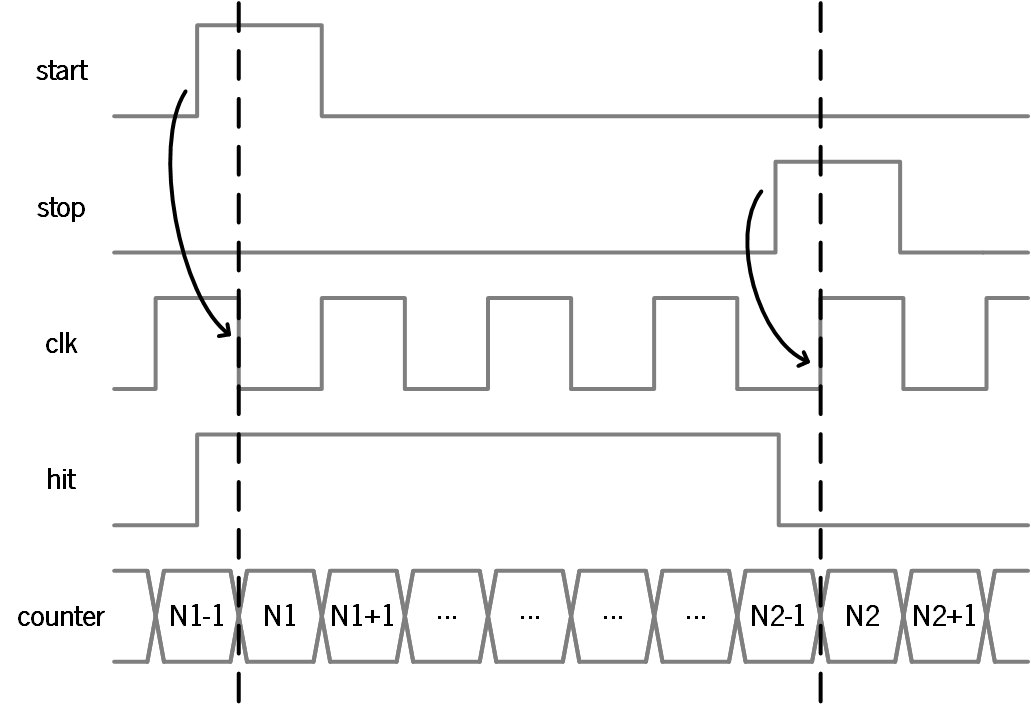
\includegraphics[width=0.6\textwidth]{img/02_StateofArt/course_conter_td.png}
	\caption{Course counter architecture waveforms. [based on \citep{course_counter_td}]}
	\label{fig:course_counter_wf}
\end{figure}

\begin{equation}
	T = (N_{2}-N{1}) * T_{clk}
	\label{eq:course_conter_measured_time}
\end{equation}

\begin{equation}
	range = 2 ^ n
	\label{eq:course_conter_range}
\end{equation}

As the performance of \glspl{FPGA} continues to improve, the maximum operating frequency also increases. In~\citep{course_counter_710}, a 710~MHz system clock (i.e., a 1.4~ns resolution) was reported to be used. Nevertheless, to achieve resolutions below some hundreds of picoseconds, a system clock frequency of 10~GHz or higher is required. For this reason, course counters should only be employed when a resolution of a few nanoseconds and a high-measurement range are required, or in combination with other architectures to improve their dynamic range with only minor hardware modifications.

When implementing this architecture, special attention must be paid to the routing of the enable signals for the sampling registers. If this is not properly considered, errors larger than 1 \gls{LSB} may occur. Counting errors can also be influenced by metastability caused by clock skew. As the clock frequency increases, the effect of the clock skew becomes more pronounced. In addiction, the increment of the number of bits of the counter makes it more challenging to achieve low clock skews between the signals fed to the counter registers.

% subsection course_counters (end)

\subsection{Phased Clocks} % (fold)
\label{sub:phased_clocks}

The main disadvantage of course counter architectural group is its limited resolution. A Phased clock \gls{TDC} reduces the \gls{LSB} to less than the sampling clock period. Phased clock architectures typically use a \gls{PLL} or a clock manager block, which are primitives of most \glspl{FPGA}. Another advantage of this architecture is its high linearity, which eliminates the need for complex calibration mechanisms to achieve good performance. Phased clocks architectures are based on two main techniques: oversampling and phase detection.

Oversampling architecture uses phased clocks as clock signals to independent course counters and the \textit{hit} signal as the counter’s enable. Basically, this architecture consists of \textit{m} course counters, where \textit{m} is the number of phase clocks used. The final measurement is calculated following equation~\ref{eq:oversampling}, where \textit{n\textsubscript{0}-n\textsubscript{m}} represents the number of counts in each counter, and \textit{T\textsubscript{clk}} is the base clock period. In~\citep{oversmapling} a \gls{PLL} was used to create a 250~MHz quadrature clock with 0-, 90-, 180- and 270-degrees, making the equivalent of a 1~GHz clock (i.e., a 1~ns resolution). When implementing this architecture, the main challenge is routing the signal to be measured with the minimum clock skew to avoid degrading measurements. Use a low-jitter \gls{PLL} to avoid phase overlap is also recommended.

\begin{equation}
	t_{oversampling} = (n_{0}+n_{1}+...+n_{n}) * \frac{T_{clk}} {m}
	\label{eq:oversampling}
\end{equation}

In Phase Detection architecture, the \textit{hit} signal is sampled with \glspl{FF} by a set of equidistant phase-shifts clocks. The higher the number of clocks phases, the higher the resolution (see equation~\ref{eq:pc_resolution}, where \textit{N\textsubscript{phases}} is the number of phases used). However, this increase in resolution also leads to more pronounced errors associated with the clock's phase generation and routing paths, which can degrade the \gls{TDC}'s linearity. Figure~\ref{fig:phase_detection_bd} depicts the basic structure of this architecture. The \textit{hit} signal is divided into four and detected by four D-type \glspl{FF}. The outputs from these \glspl{FF} are aligned step by step in the chains of additional \glspl{FF}, where metastable states are suppressed, creating a common clock domain for further measurement code processing. This synchronization step will be as large as the number of phases used. Figure~\ref{fig:phase_detection_wf} shows a waveform diagram of an \textit{hit} signal and the quad-phase clocks. A rising edge is detected and the timing is extracted from the pattern "0111". The main challenge while implementing this architecture is related to the jitter associated with the different phases that degrade the \gls{TDC}'s' performance. The jitter values from the phase shift generators and the routing skew can lead to situations where the \textit{n} phase clock rising edge arrives before the \textit{n} – 1 phase-clock rising edge, creating a code pattern with bubbles. In~\citep{phase_det} a 280~ps \gls{TDC} based on phase detection with a \gls{DNL} of less than half of a system \gls{LSB} was reported.

\begin{figure}[ht!]
	\centering
	\begin{subfigure}[b]{0.95\textwidth}
		\centering
		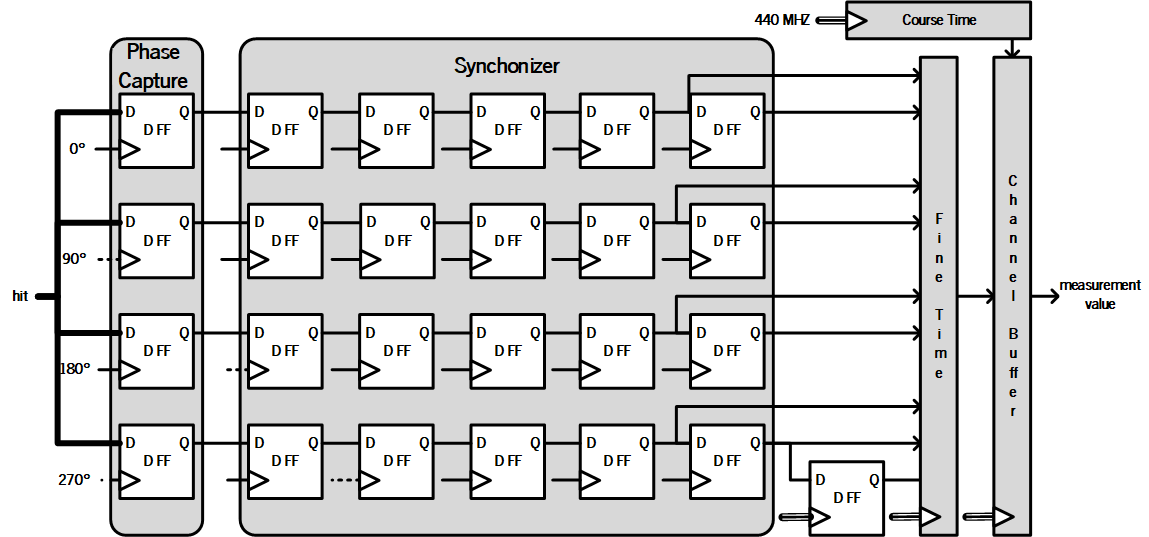
\includegraphics[width=\textwidth]{img/02_StateofArt/phase_detection.png}
		\caption{}
		\label{fig:phase_detection_bd}
	\end{subfigure}
	\begin{subfigure}[b]{.5\textwidth}
		\centering
		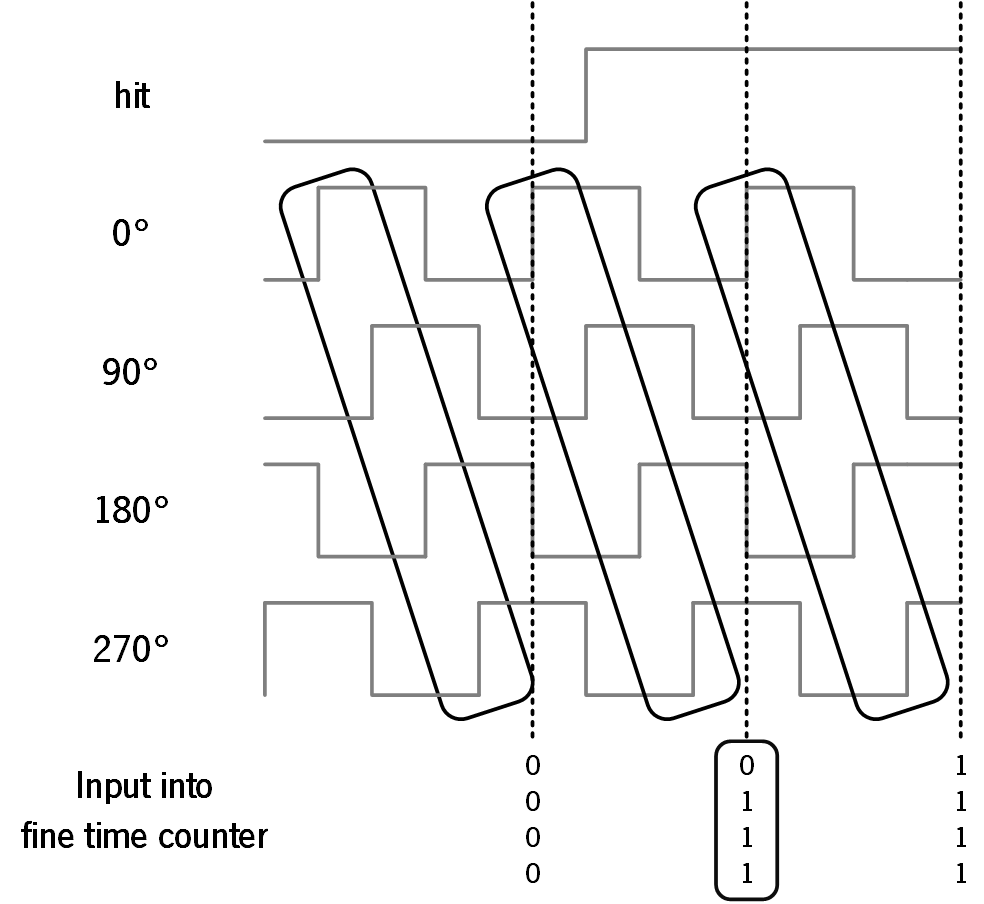
\includegraphics[width=\textwidth]{img/02_StateofArt/phase_detection_wf.png}
		\caption{}
		\label{fig:phase_detection_wf}
	\end{subfigure}
	\caption{Phase detection architecture: (a) block diagram; (b) waveform diagram (adapted from \citep{phase_det}).}
	\label{fig:phase_detection}
\end{figure}

\begin{equation}
	\tau = \frac {T_{clk}} {N_{phases}}
	\label{eq:pc_resolution}
\end{equation}

% subsection phased_clocks (end)

\subsection{Tapped-Delay Lines} % (fold)
\label{sub:tapped_delay_lines}

\Acrlongpl{TDL} are the most widely employed technique to realize high-resolution \glspl{TDC}. \Glspl{TDC} based on this architecture can achieve picosecond resolutions, which is significantly higher than what is possible with counter-based architectures. The the basic structure of a \gls{TDL}-\gls{TDC} is shown in figure~\ref{fig:tdl_bd}. The input stage is often used to manipulate the \textit{hit} signal to make it easier for the rest of the system to handle and to increase the system's resolution. The manipulated \textit{hit} signal is then propagated along the delay line for time interpolation. The \gls{TDL} status is latched out by the sample stage which outputs a thermometer code. This code is then interpreted by a thermometer-to-binary decoder to produce the interpolator timestamp. The decoding stage can have a significant impact on the \gls{TDC}’s dead time. The thermometer code is as big as the \gls{TDL}’s number of delay elements. A \gls{TDL} implemented in \gls{FPGA} can easily reach a few hundred logic cells. The decoding block will, therefore, be composed of multiple stages of combinational blocks. If no special care is taken, the time needed to reach a conversion can surpass the system clock cycle. To minimize the system’s nonlinearities, a calibration block is often implemented.

\begin{figure}[ht!]
	\centering
	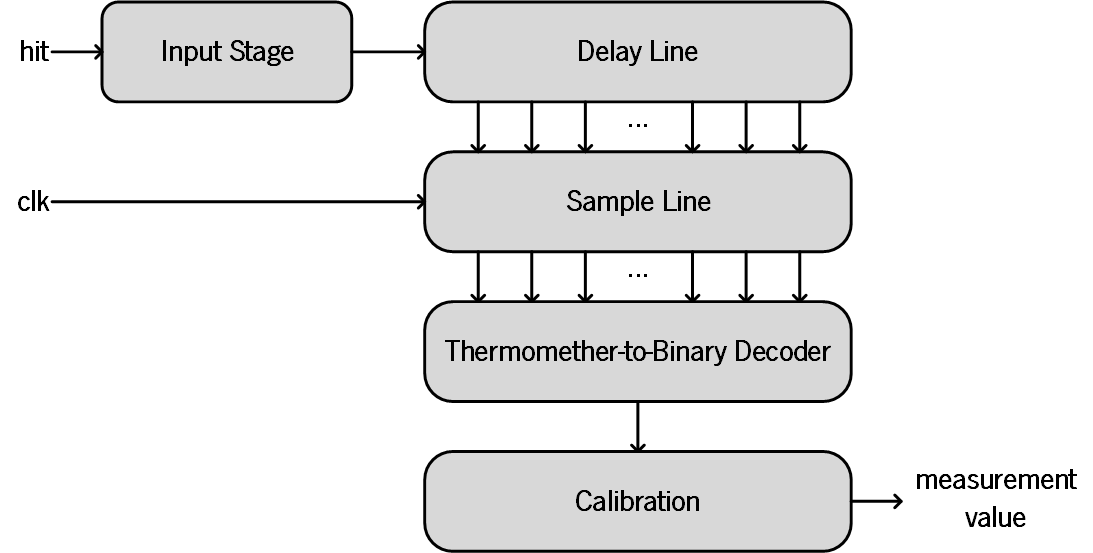
\includegraphics[width=0.6\textwidth]{img/02_StateofArt/tdl_block.png}
	\caption{TDL-TDC block diagram (adapted from \citep{machado_ov}).}
	\label{fig:tdl_bd}
\end{figure}

Figure~\ref{fig:tdl_architecture} presents the basic architecture of the delay line, which is the core of the \gls{TDL} architecture. TThe delay line must ensure that the full measurement range is covered. Usually, the stop signal is the system clock. Therefore, the delay line must be long enough to comprise an entire clock cycle. The maximum achievable resolution by a \gls{TDL} is determined by the intrinsic delay value of the cells used to build the delay line. For a single \gls{TDL} channel, the time interval measure value can be calculated according to equation~\ref{eq:tld}, where $\tau$ is the propagation delay of each element and \textit{n} is the number of cells traversed by the delayed signal. In \gls{FPGA} platforms, the most used delay elements are the carry chains cell primitives, as they have a dedicating routing with the smallest internal propagation delay. However, there are research works that employed \gls{LUT} cells primitives \citep{tdl_lut} and \glspl{FF} \citep{tld_ff} to build the delay line.

\begin{figure}[ht!]
	\centering
	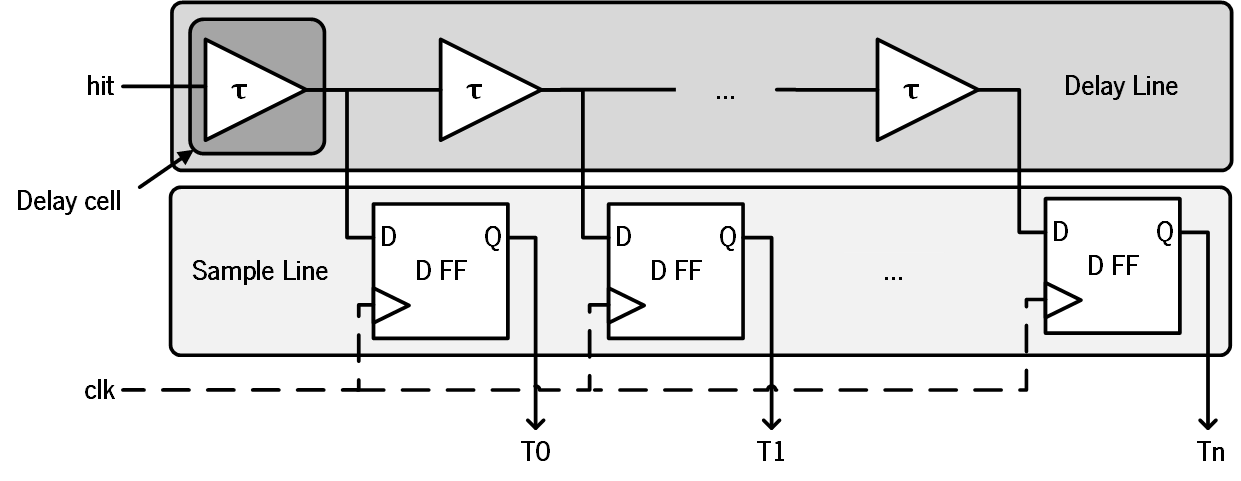
\includegraphics[width=0.7\textwidth]{img/02_StateofArt/tdl_architecture.png}
	\caption{TDL architecture.}
	\label{fig:tdl_architecture}
\end{figure}

\begin{equation}
	t_{fine} = n * \tau
	\label{eq:tld}
\end{equation}


As \gls{FPGA} manufacturing technology improves, the intrinsic propagation delay of the cells used to build the delay line becomes smaller. This, combined with the \gls{TDL}-\gls{TDC} operation principle, suggests that a \gls{TDL} implemented in a \gls{FPGA} made with more advanced processing technology should naturally improve its precision. However, this is not necessarily true. The \textit{hit} signal should transmit sequentially from one delay element to the next one, and be sampled by the bank of registers according to the its hard-wired connection, as shown in figure~\ref{fig:no_bubble}. However, the sampling clock that reaches each sample stage \gls{FF} is not simultaneous, which makes the order of real delays times in the taps inconsistent with the order of their physical locations, leading to bubble codes (see figure~\ref{fig:bubble}). This problem is particularly evident in \glspl{FPGA} made with 28~nm and more advanced technologies \citep{wu_first}. As the tap intervals become shorter, the bubbles become more severe. There are several solutions to address this problem. One solution consists of reordering the taps \citep{bin_realigment}, which can minimize the bubble occurrence and reduce the complexity of decoding stage. This is typically done with the help of a histogram to detect zero delay cells. \citet{tuned_line} proposed a bin-width tuning method that involves adjusting the \textit{hit} transitions and sample patterns of the carry chain while taking into account the delays of the sum and carry-out bins. This method can improve the uniformity of the bin width, resulting in improved measurement precision. Another approach consists of counting the number of “1” in the \gls{TDL} instead of determining the \gls{TDL}'s bin in which the signal transition occurs \citep{count_ones}. This method produces the same result as determining the position of the \textit{hit}, with the advantage of allowing the bubble occurrences to be ignored.

\begin{figure}[ht!]
	\centering
	\begin{subfigure}[b]{.35\textwidth}
		\centering
		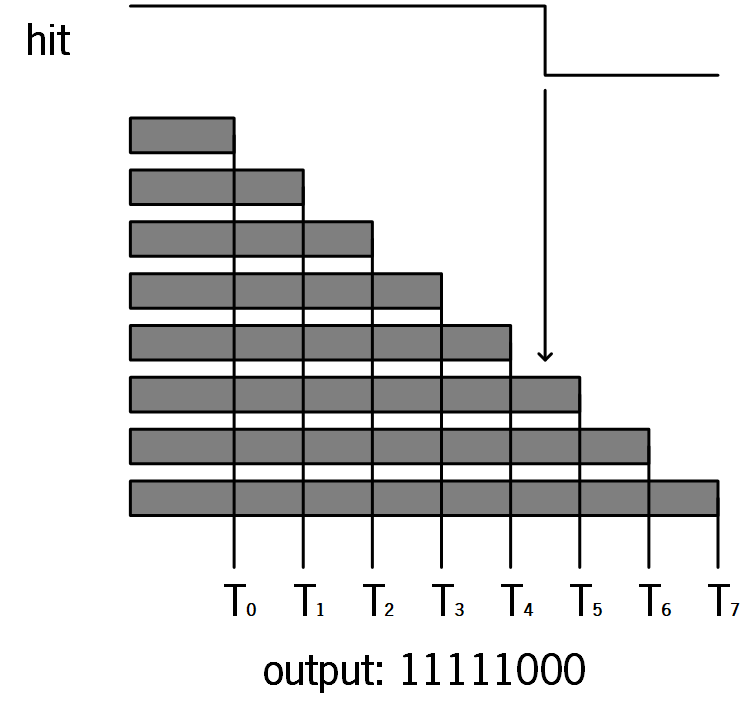
\includegraphics[width=\linewidth]{img/02_StateofArt/no_bubble.png}
		\caption{}
		\label{fig:no_bubble}
	\end{subfigure}
	\begin{subfigure}[b]{.35\textwidth}
		\centering
		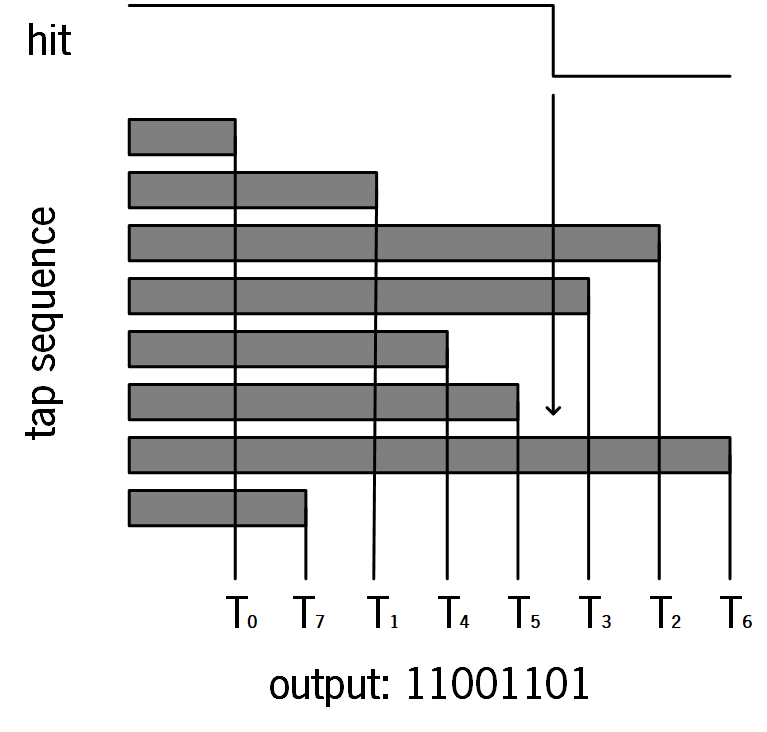
\includegraphics[width=\linewidth]{img/02_StateofArt/bubble.png}
		\caption{}
		\label{fig:bubble}
	\end{subfigure}
	\caption{TDL output: (a) tap sequence consistent with the order of the real delay time of cells; (b) tap order not consistent with the order of the real delay time of cells (adapted from \citep{count_ones}).}
	\label{fig:bubble_diagram}
\end{figure}

In many \gls{TDC} applications, the resolution is limited by the presence of ultra-wide bins, which are significantly wider quantization steps that occur due to the grain architecture and clock distribution scheme of \glspl{FPGA}. Constraining the length of the entire delay line to a single basic logic block can help to alleviate ultra-wide bins problems, but this requirement is impossible to accomplish in a practical \gls{TDC} design since the fine time interpolator must cover an entire period of the system clock. A novel method called \gls{WU} \gls{TDC}, proposed by \citet{wu_first} in \citeyear{wu_first}, significantly reduces the bin width. \gls{WU} launchers are design to make multiple measurements with a single delay structure, effectively subdividing the ultra-wide bins in each measurement. Figure~\ref{fig:wu_bd} presents the basic structure of the traditional \gls{WU} \gls{TDC}. The measurements of the multiple transitions reduce the nonlinearities in the delay line, improving the overall performance of the \gls{TDC}, although increasing dead time and requiring a more complex decoder scheme. In~\citep{wu_ex}, a \gls{WU}-A \gls{TDC} achieved a 1.77~ps resolution and a 3.0~ps precision. In \citeyear{wu_not_suitable_ultrascalte}, \citet{wu_not_suitable_ultrascalte} concluded that \gls{WU} \glspl{TDC} were not suitable for improving time precision due to bubble errors in UltraScale \glspl{FPGA}. Therefore, during many years there were no efficient \gls{WU} \gls{TDC} reported to such devices. Only in \citeyear{wu_novel_ultrascale}, an efficient \gls{TDC} in 20~nm \glspl{FPGA} with \gls{WU} methods was proposed by \citet{wu_novel_ultrascale}. The authors conclude that the \gls{WU} methods are still efficient in improving the resolution with maintained linearity in UltraScale \gls{FPGA} when a sub-\gls{TDL} structure is also integrated. By combining a \gls{DS} structure, the \gls{WU} method and the sub-\gls{TDL} architecture a \gls{DS}\gls{WU} \gls{TDC} with 1.23~ps resolution was implemented. A brief review of wave union \glspl{TDC} can be found in \citep{wu_brief_review}.

\begin{figure}[ht!]
	\centering
	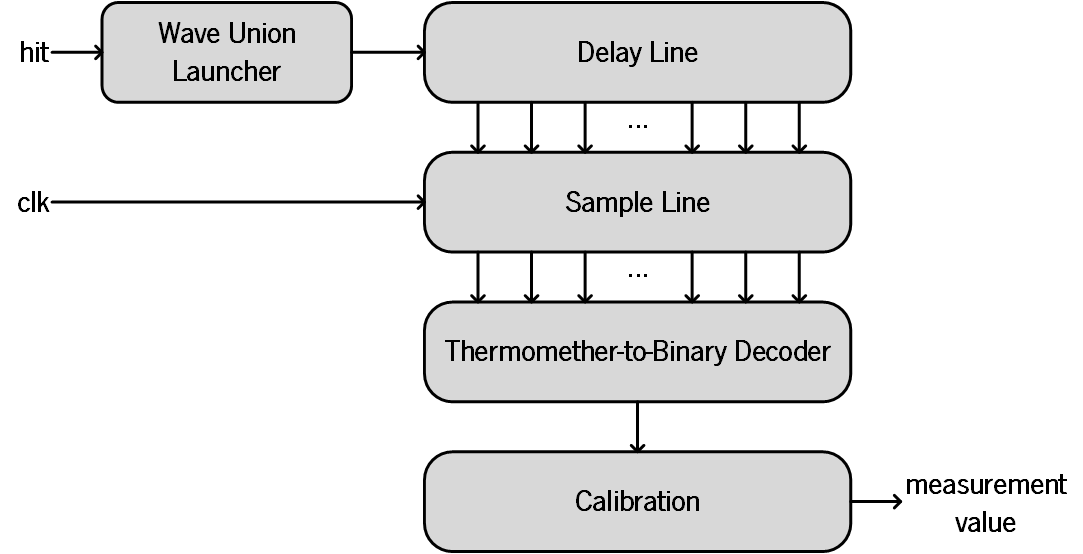
\includegraphics[width=0.6\textwidth]{img/02_StateofArt/wu.png}
	\caption{Traditional WU block diagram (adapted from \citep{wu_brief_review}).}
	\label{fig:wu_bd}
\end{figure}

The non-uniformity of delay elements in the \gls{TDL} caused by manufacturing process technology and ultra-wide bins is another considerable problem. In literature there are two main solutions to mitigate this issue: bin-by-bin calibration and bin decimation. Bin-by-bin calibration \citep{bin_by_bin_calibration} is more suitable for \glspl{TDC} with higher linearity and resolution requirements. It consists of a statistical approach and it is performed through code density tests. To perform this test, a periodic signal with frequency that is unrelated to the system clock frequency should be chosen as the \textit{hit} signal. The results from multiple measurements are recorded together with the last cell to be sampled. Considering that every cell on the delay line has the same propagation delay, and because the frequency of the \textit{hit} signal is unrelated to the frequency of the system clock, the probability for each cell to be the last one to be sampled is the same. These measurements results can be represented in a histogram, and an estimate of the cells’ actual delay can be obtained by using equation~\ref{eq:cell_delay}, where $\tau$\textit{\textsubscript{i}} is the \textit{ith} cell’s delay, \textit{n\textsubscript{i}} is the number of times the \textit{ith} delay cell was recorded, \textit{T\textsubscript{clk}} is the system clock period, and \textit{N} is the number of measurements performed. This histogram is stored in an embedded \gls{RAM} to calibrate the \gls{TDC} measurements during its operation. In bin decimation \citep{bin_decimation}, the linearity of the \gls{TDL} can be improved at the cost of resolution. This solution also achieves good results when multiple \glspl{TDL} are used, as it does not increase the utilization of hardware resources. It consists of a reorganization of the current bins into several groups bins as a new one. The purpose is to minimize the \gls{INL} of the new line enabling the achievement of bins with more uniform sizes, increasing the linearity of the chain so that bin-by-bin calibration may not be needed. A less usual technique based on load-regulation technique in proposed in \citep{hw_linearization}. The load regulation depends on connecting an appropriate number of unused three-state-buffers or \gls{CLB} inputs to the wire which delay is adjusted. Depending on the number of inputs connected to the wire, its capacitance changes which influences its time-constant and finally changes its time delay. This method considerably uses fewer resources than bin-by-bin calibration technique at a cost of a more complex implementation.

\begin{equation}
	\tau_{i} = n_{i} * \frac{T_{clk}}{N}
	\label{eq:cell_delay}
\end{equation}

To improve the resolution and linearity of \gls{TDL}, multiple-chain \gls{TDL} architectures can be used. In this architecture, the \textit{hit} signal is propagated through the parallel chains simultaneously, and the arrival time is measured \textit{N} times, where \textit{N} is the number of parallel carry chains. The \gls{TDC} resolution can be theoretically improved by a factor of $\sqrt{N}$ compared to a single chain \gls{TDC} \citep{pvt_mc}. Additionally, different \glspl{TDL} implementations in the same \gls{FPGA} will have different transfer curves. Averaging the different thermometer codes obtained from the different chains reduces the ultra-wide bins effect increasing the overall \gls{TDC} linearity, as illustrated in figure~\ref{fig:multiple_chain_td}. In~\citep{pvt_offset} a multiple-chain \gls{TDC} with 20 carry chains was implemented achieving a 1.15~ps resolution and a 3.5~ps precision. The disadvantage of multiple-chain architecture is related to the resources utilization since each \gls{TDL} requires a considerable amount of resources. When implementing this architecture, the routing of the \textit{hit} signal must be done in a way that the offset between channels is minimized.

\begin{figure}[ht!]
	\centering
	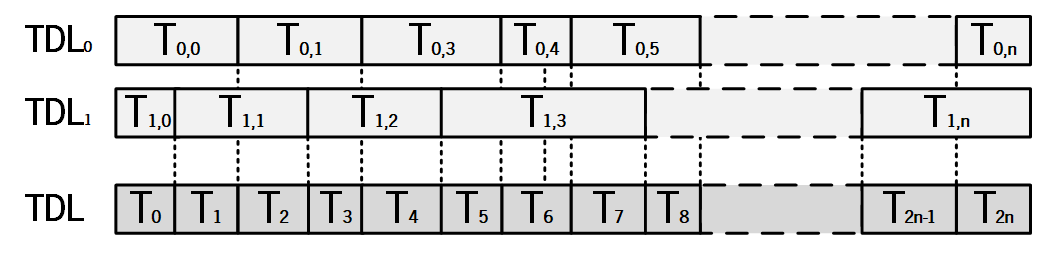
\includegraphics[width=.7\textwidth]{img/02_StateofArt/ultrawide_bin.png}
	\caption{Reduction of ultra-wide bins effect (adapted from \citep{tdl_hyb_1.9}).}
	\label{fig:multiple_chain_td}
\end{figure}

The delay time of a carry chain is also sensitive to \gls{PVT} conditions. Thus, the measurement precision and resolution can deteriorate due to voltage and temperature \citep{pvt_offset}. Solutions to this problem will be addressed in subsection~\ref{sec:self_calibration_mechanisms}.

A recent trend is to pair a \gls{TDL} with phase clocks architectures to shrink the \gls{TDL} length, reducing hardware utilization and the effects of nonlinearities. Because the effects of nonlinearities are propagated through the delay line, it is desirable to have a delay line as short as possible. This architecture is based on a two-stages interpolation within a single period of the system clock signal. Figure~\ref{fig:tld_bybrid_wf} shows the measurement of a time interval by this architecture, where a \gls{FPC} is used. The first interpolation stage involves the use of phased clock to detect the nearest edge of the phased clock after the start and signals arrive. Since the widths of the phase clock time segments are known \textit{T\textsubscript{ST1}} and \textit{T\textsubscript{SP1}} can be calculated accurately. The second interpolation stage uses a \gls{TDL} to cover the period between two phases of the phased clocks, \textit{T\textsubscript{ST2}} and \textit{T\textsubscript{SP2}}. The fine measure is calculated following equation~\ref{eq:tdl_hybrid}. Hybrid \glspl{TDL} using eight-clock and four-clock phases achieved resolutions of 1.9~ps and 2.9~ps in \citep{tdl_hyb_1.9} and \citep{tdl_hyb_2.9}, respectively.

\begin{figure}[ht!]
	\centering
	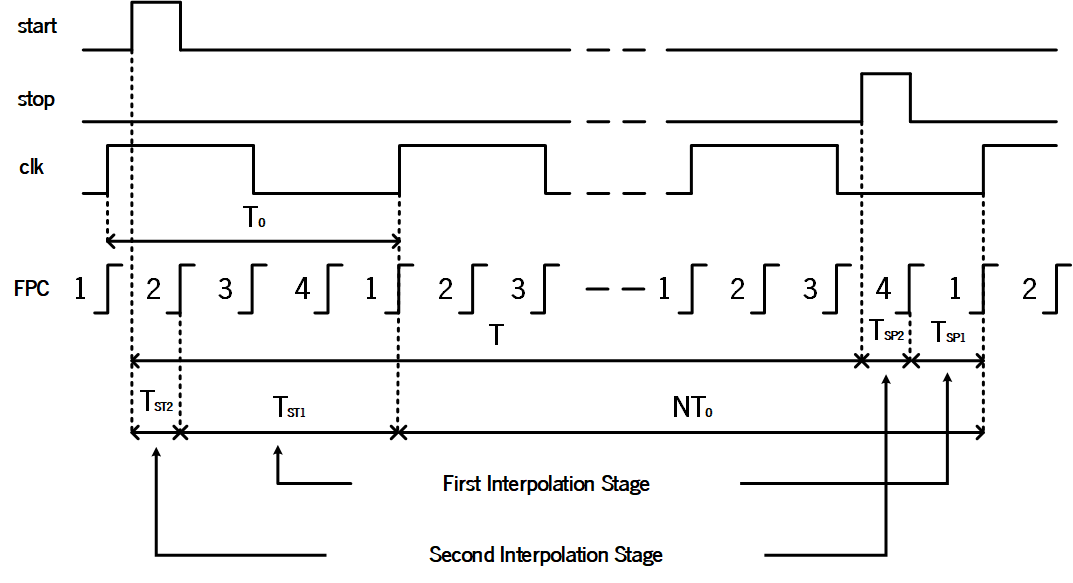
\includegraphics[width=.7\textwidth]{img/02_StateofArt/tld_hybrid_wf.png}
	\caption{Hybrid TDL waveforms (adapted from \citep{tdl_hyb_2.9}).}
	\label{fig:tld_bybrid_wf}
\end{figure}

\begin{equation}
	t_{fine} = (T_{ST1} + T_{ST2}) - (T_{SP1} + T_{SP2})
	\label{eq:tdl_hybrid}
\end{equation}

% subsection tapped_delay_lines (end)

\subsection{Differential Delay Lines} % (fold)
\label{sub:differential_delay_lines}

The maximum achievable resolution of \gls{TDL} architectures is limited by the intrinsic delay of the individual cells, and cannot be improved beyond this limit. To overcome this limitation, differential \gls{TDC} architectures were proposed. Differential delay lines can be implemented using \acrlongpl{TDL} and \glspl{RO}, and can provide picosecond time resolution when carefully designed and operated.

The 2-D \gls{TDL} architecture is a variation of the traditional \gls{TDL} architecture that uses two delay lines with different intrinsic cell delays for both the start and stop signals. This allows for a higher resolution time measurement, as the resolution is determined by the difference between the two delay elements rather than the absolute value of a single delay element (see equation~\ref{eq:2tdl_resolution}, where $\tau$\textit{\textsubscript{1}} and $\tau$\textit{\textsubscript{2}} are the propagation delay of each delay element of slow and fast delay lines, respectively). Figure~\ref{fig:2tdl} presents a schematic of a 2-D \gls{TDL} architecture. The fine measure is calculated according to equation~\ref{eq:2tdl_measure}, where \textit{n} is the number of the traversed delay elements of the slow delay line. In order to accurately measure the time difference, it must be guaranteed that the clock delay chain has a shorter propagation delay than the hit delay chain, so that the \textit{clk} signal can catch up to the \textit{hit} signal. Otherwise, the \textit{clk} signal will never be able to catch up with the \textit{hit} signal and the \gls{TDC} will always return the maximum value. In \gls{FPGA} platforms, the limited range of available cells with different delays can make it challenging to implement this architecture. The same cell can be used to both start and delay chains and the difference between each stage of the two delay lines is obtained by their routing. The 2-D \gls{TDL} architecture suffers from the same problems as the \gls{TDL} architecture. The delay line tends to be much larger than in the normal \gls{TDL} architecture, increasing the resources usage and nonlinearities across the chain. These problems cause \gls{RO} implementations to be more popular than 2-D \gls{TDL} architecture regarding to \gls{FPGA} platforms. Nevertheless, in \citep{2tdl_ex} a 2-D \gls{TDL}, based on \gls{FPGA} internal routing resources, achieved a 9~ps resolution and a 6.5~ps precision.

\begin{figure}[ht!]
	\centering
	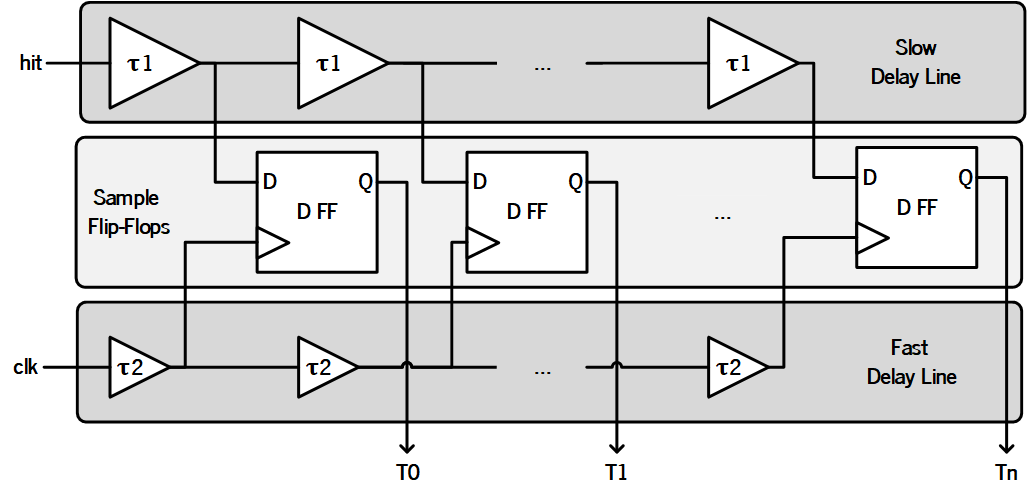
\includegraphics[width=.7\textwidth]{img/02_StateofArt/2dtdl.png}
	\caption{Differential delay line architecture (adapted from \citep{2tdl_bd}).}
	\label{fig:2tdl}
\end{figure}

\begin{equation}
	\tau = \tau_{1} - \tau_{2}
	\label{eq:2tdl_resolution}
\end{equation}

\begin{equation}
	t_{fine} = n * \tau
	\label{eq:2tdl_measure}
\end{equation}

The \gls{RO} architecture is a type of differential delay line that uses a dual \glsentrylong{RO} schema paired with a coincident detector. The resolution of the \gls{TDC} is given by the difference in frequency between the two oscillator (see equation~\ref{eq:ro_resolution}, where \textit{T\textsubscript{1}} and \textit{T\textsubscript{2}} correspond to the slow and fast oscillators' periods, respectively). This architecture solves the cell delay mismatch issue that can affect delay line architectures, since the resolution is no longer dependent on the intrinsic delay of individual cells. The \gls{RO} architecture is essentially a \gls{TDL} whose output loops back to its input, allowing for repeated measurements of the same time interval. Smaller \gls{DNL} and \gls{INL} will be obtained due to the disappearance of the ultra-wide bins \cite{ro_bi_interpolation}. However, the \gls{RO} architecture can be more complex to implement and require more resources than a \gls{TDL}. There are two main variants of \gls{RO}-\gls{TDC}: \glspl{RO} with two independent counters and \glspl{RO} with a single counter. The use of two independent counters allows for more flexibility and better performance, but requires more resources. In contrast, \glspl{RO} with a single counter are simpler to implement and require fewer resources, but may have lower performance.

\begin{equation}
	\tau = T_{1} - T_{2}
	\label{eq:ro_resolution}
\end{equation}

The \gls{RO} architecture with two independent counters uses two counters, each incremented by one of the oscillators, and a coincident detector \citep{ro_2_counter}. The block and waveform diagrams of this architecture are illustrated in figure~\ref{fig:ro_2_cnt}. The measure time interval for this architecture is given by equation~\ref{eq:ro_2cnt_measure}, where \textit{n\textsubscript{1}} and \textit{n\textsubscript{2}} correspond to the slow and fast counter's values, respectively. The \gls{RO} architecture with a single counter employs only one counter that is clocked by the slow oscillator and stops counting once the fast oscillator can surpass it \citep{ro_1_counter}. Figure~\ref{fig:ro_1_cnt} depicts this variant architecture. The pulse width reshaping module is responsible to regenerate the pulse width to a constant value so that it can sustain stable oscillation, and the ctrl2generator module is used to indicate the proper latching moment for the fine counter content. In~\citep{ro_2_counter}, a \gls{RO} with two counter achieved a resolution of 3~ps. In~\citep{2tdl_bd}, a \gls{RO} with a single counter achieved a resolution of 31~ps and a maximum dead time value of 256~ns.

One advantage of \gls{RO} architecture is that it can directly obtain a fine time by reading the content of the counter, which is a natural binary code, without the need for a decoder. The fine measure is obtained from equation~\ref{eq:ro_1cnt_measure}, where \textit{n\textsubscript{fine}} is the number of counts in the counter until the fast oscillator is able to overtake the slow one. The greatest disadvantage of \gls{RO} architecture is related to its dead time that can reach several microseconds, which limits the maximum measurement rate of the system. According to equation~\ref{eq:ro_2cnt_max_cnt}, this problem can be surpassed by decreasing the \gls{TDC} resolution, which is not desirable, or by increasing the oscillation frequency.

\begin{figure}[ht!]
	\centering
	\begin{subfigure}{.49\textwidth}
		\centering
		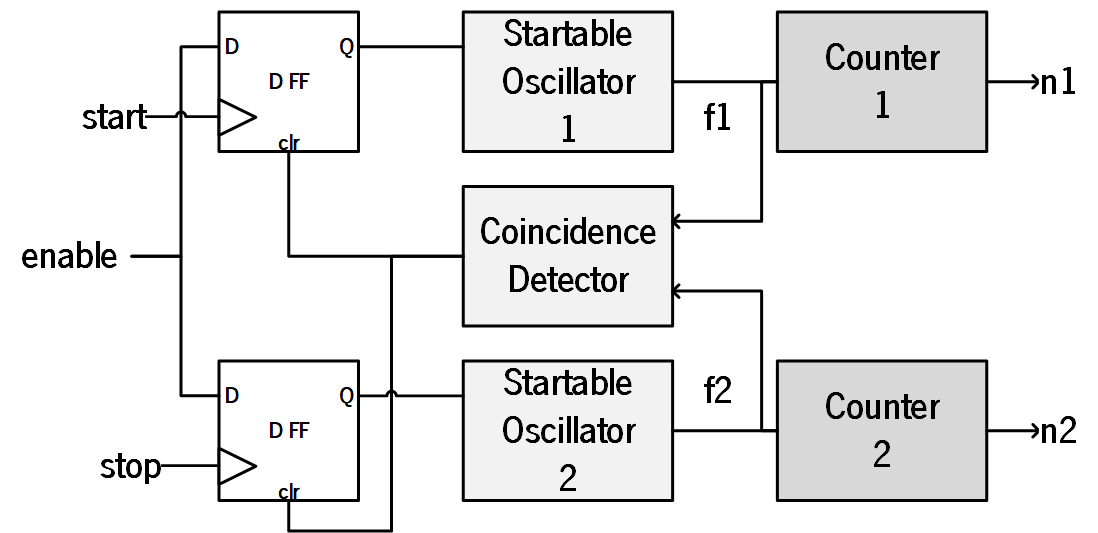
\includegraphics[width=\linewidth]{img/02_StateofArt/RO_2cnt_bd.png}
		\caption{}
		\label{fig:ro_2_cnt_bd}
	\end{subfigure}
	\hfill
	\begin{subfigure}{.49\textwidth}
		\centering
		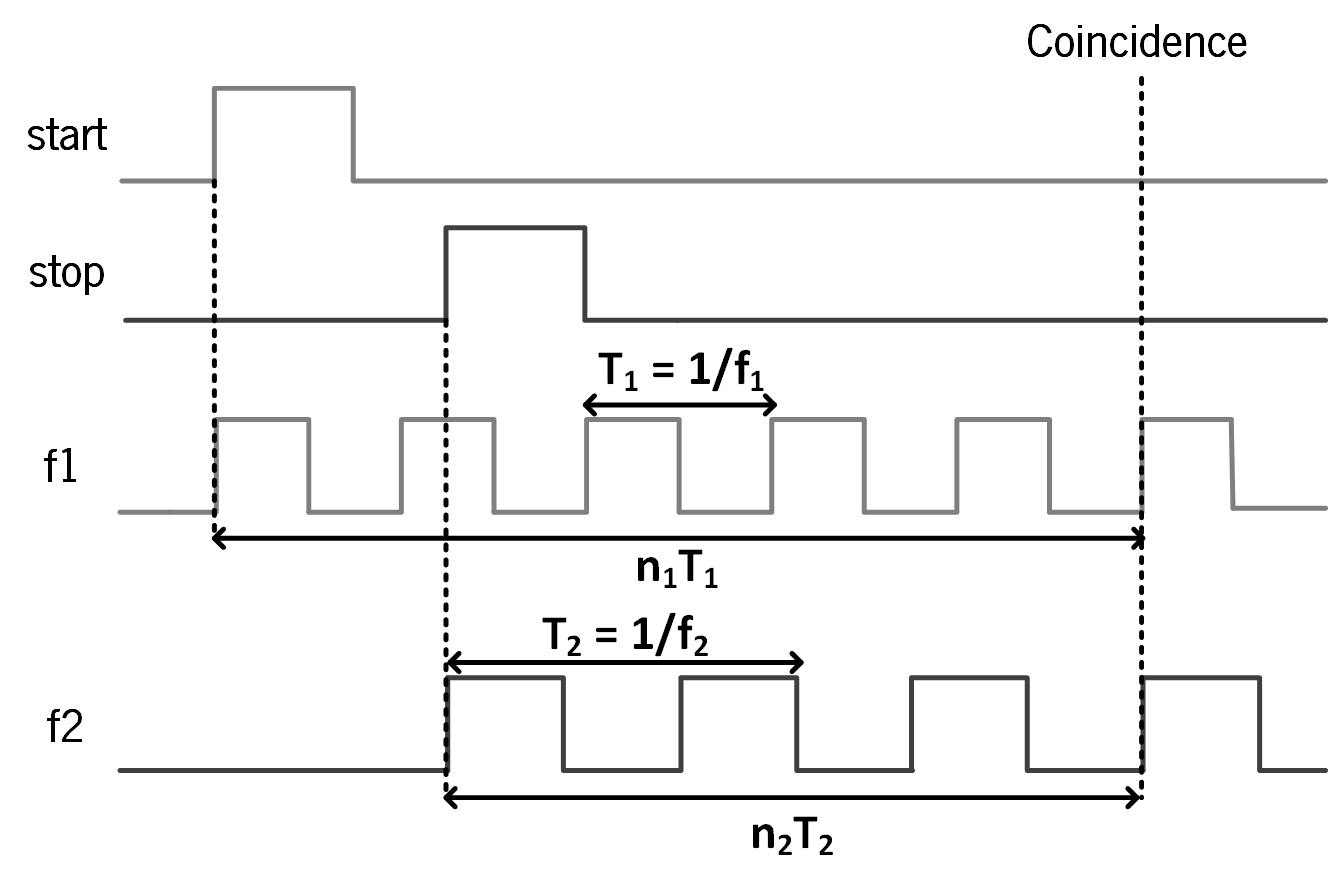
\includegraphics[width=\linewidth]{img/02_StateofArt/ro_2cnt_wf.png}
		\caption{}
		\label{fig:ro_2_cnt_wf}
	\end{subfigure}
	\caption{RO with two independent counters: (a) block diagram; (b) waveform diagram (adapted from \citep{ro_2_counter}).}
	\label{fig:ro_2_cnt}
\end{figure}

\begin{equation}
	t_{two\_counters} = (n_{1} - 1) * T_{1} - (n_{2} - 1) * T_{2}
	\label{eq:ro_2cnt_measure}
\end{equation}

\begin{figure}[ht!]
	\centering
	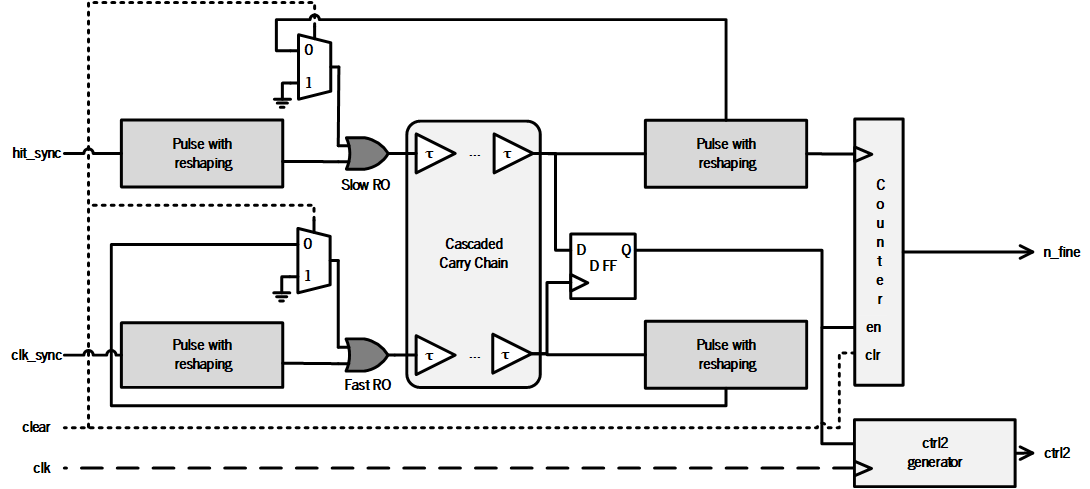
\includegraphics[width=.9\textwidth]{img/02_StateofArt/RO_1cnt .png}
	\caption{RO with a single counter (adapted from \citep{ro_1_counter}).}
	\label{fig:ro_1_cnt}
\end{figure}

\begin{equation}
	t_{one\_counter} = n_{fine} * \tau
	\label{eq:ro_1cnt_measure}
\end{equation}

\begin{equation}
	t_{max\_counv} = \frac {T_{1} - T_{2}} {\tau}
	\label{eq:ro_2cnt_max_cnt}
\end{equation}

In \citeyear{ro_bi_interpolation}, \citet{ro_bi_interpolation} proposed a novel approach that uses a bi-time interpolation scheme to address resolution problems without adding extra resource consumption and dead time. This approach uses the system clock as a reference and only requires one ring oscillator, which can help avoid factors that cause metastability and reduce resource consumption. To integrate this architecture in the taxonomy proposed in \citep{machado_ov}, and following the authors' approach, a new sub-architecture named hybrid is included in differential delay lines architectural group. The bi-time schema for fine time interpolation is illustrated in figure~\ref{fig:ro_bi_interpolation}. The phased clock module uses a \gls{FPC} (as present in subsection~\ref{sub:phased_clocks}). The \acrlong{RO} module is composed by a \gls{RO}, a counter, and a coincidence detector circuit. The \gls{RO} is triggered by the \textit{hit} signal to start oscillation. The rising edge of the oscillation signal will gradually moves from one region of the clock signal to an adjacent one. The coincidence detector circuit determines whether the rising edge of the oscillation signal crosses over any region boundaries of the clock signal. The counter value indicates the period difference between the oscillation signal and the reference clock signal. The proposed approach achieved a time resolution of 20~ps, dead time of 58~ns, and a precision of 15~ps to 20~ps.

\begin{figure}[ht!]
	\centering
	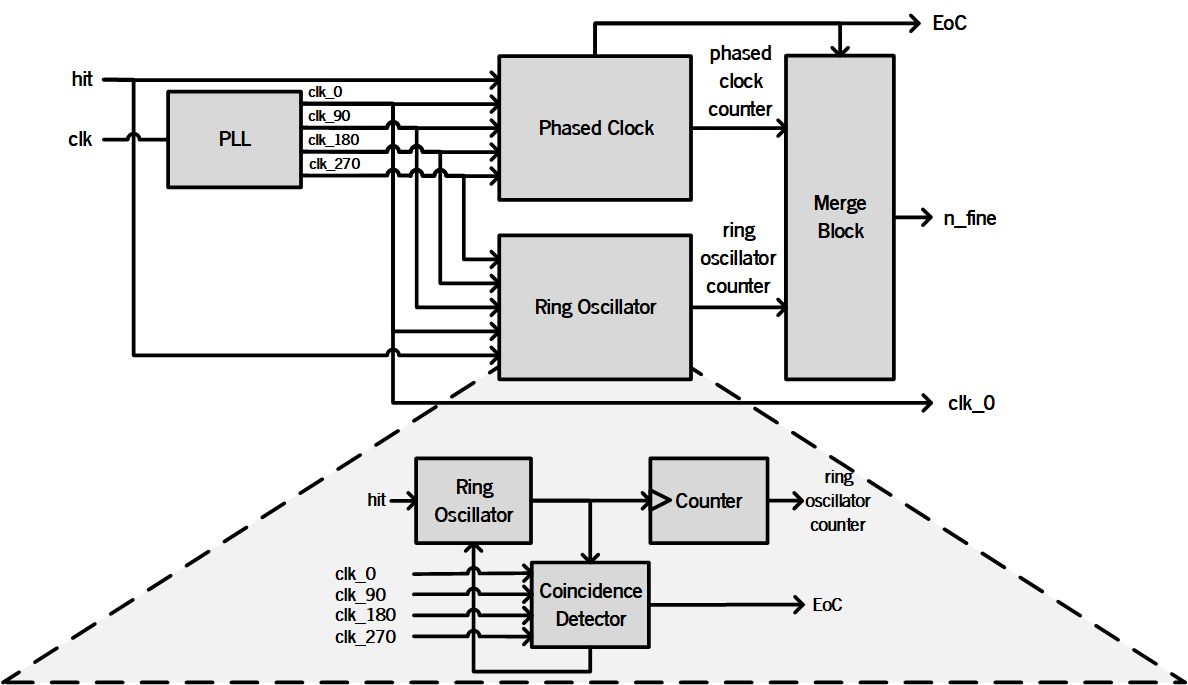
\includegraphics[width=0.9\textwidth]{img/02_StateofArt/RO_hybrid.png}
	\caption{Hybrid differential delay line (adapted from \citep{ro_bi_interpolation}).}
	\label{fig:ro_bi_interpolation}
\end{figure}

% subsection differential_delay_lines (end)

\subsection{Pulse-Shrinking} % (fold)
\label{sub:pulse_shrinking}

The principle of operation of pulse-shrinking \glspl{TDC} is based on the delay cells' rising and falling times' mismatch. The basic idea is to construct a propagation delay line such that the time its takes for a signal to go from low to high (\textit{T\textsubscript{PHL}}) is greater than that the time it takes to go from high to low (\textit{T\textsubscript{PLH}}). As a result, the time pulse shrinks as it cycles through the delay line. Figure~\ref{fig:pulse_shrinking} depict the concept of cyclic pulse shrinking. The pulse width can be calculated using equation \ref{eq:pulse_shrinking_measure}, where \textit{n} is the number of cycles taken until the pulse disappears. This number is proportional to the original time pulse. The minimum resolution corresponds to the amount of time the pulse shrinks per cycle.

\begin{figure}[ht!]
	\centering
	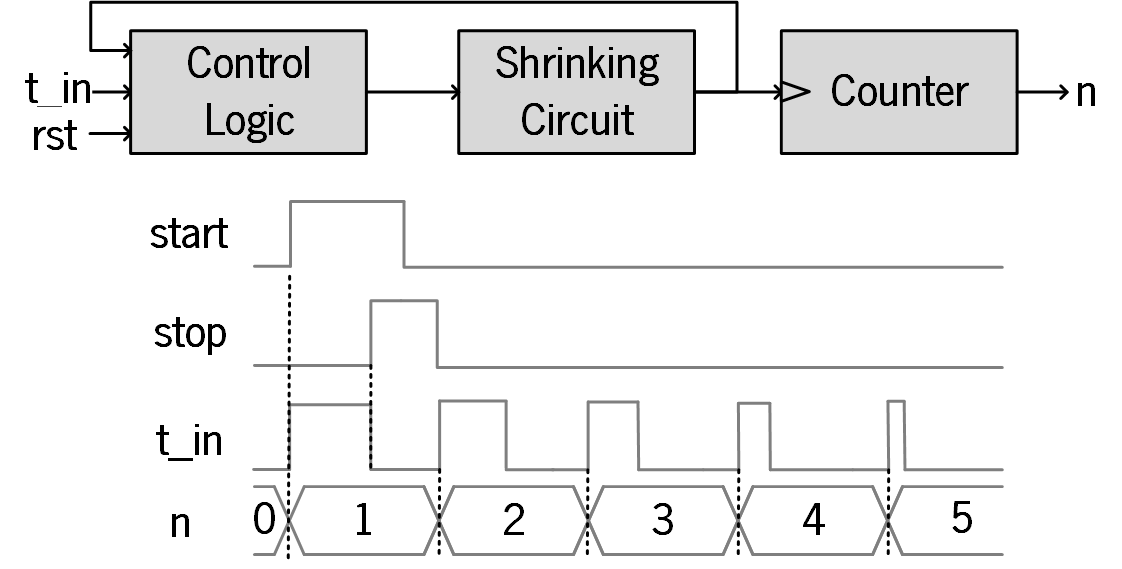
\includegraphics[width=.6\textwidth]{img/02_StateofArt/pulse_shrinking.png}
	\caption{Pulse shrinking principle (adapted from \citep{mattada_ov}).}
	\label{fig:pulse_shrinking}
\end{figure}

\begin{equation}
	t_{in} = n * (t_{PLH} - t_{PHL})
	\label{eq:pulse_shrinking_measure}
\end{equation}


The main disadvantage of pulse-shrinking architecture is that it can suffer from measurement offset when the input pulse becomes too narrow, resulting in an invalid output signal. This can limit the accuracy of the measurement. To overcome this issue, wide dynamic range and improve precision, ~\citet{pulse_shrinking_offset} proposed a pulse-shrinking variant using offset error cancellation circuitry. \citet{pulse_shrinking} reported a pulse-shrinking \gls{TDC} with a 2.38~ps resolution and both \gls{DNL} and \gls{INL} less than a quarter of \gls{LSB}. However, the measure range is limited to 80~ps.

Pulse-shrinking \gls{FPGA}-based \glspl{TDC} have several advantages, such as low resource usage and high precision. However, they are only suitable for single-shot and low-sampling rate applications \citep{mattada_ov}. In fact, \citet{machado_ov} do not consider pulse-shrinking architectures to be a promising approach for high-performance \glspl{FPGA}-based time measurement systems. These limitations should be considered when choosing a pulse-shrinking \gls{TDC} for a specific application.

% subsection pulse_shrinking (end)

\subsection{Gray Code} % (fold)

Modern applications demanding for multiple \gls{ToF} measurement channels require not only high performance but also low resource and power consumption. In fact, there are applications such as mobile and wearable devices where resources and power concerns are prioritized over resolution.

In \citeyear{gray_code_first}, \citet{gray_code_first} introduced a novel architecture that focuses on low power consumption and low resource usage, while offering high scalability and portability. The proposed architecture achieved a resolution ranging from 256~ps to 271~ps for the two \gls{TDC} channels implemented, and a 160~ps precision using only 8 \glspl{LUT} and 8 \glspl{FF} per channel. The proposed \gls{TDC}, illustrated in figure \ref{fig:gray_code_fisrt}, consists of two primary parts: a combinatorial gray code oscillator and D-type \glspl{FF} for sampling. The combinatorial stage is responsible to calculate the next value in the count schema, while the sampling stage is responsible for latching the value of the counter at each clock cycle, ensuring a stable value for the combinatorial stage, so that the next value can be correctly calculated and latched in the next clock cycle. The sequence generator is not driven by a periodic clock. In gray code sequence, there is only a single bit transition between two consecutive states. Since only a path is relevant at a time, the difference of propagation delays in various feedback paths is not harmful, so the combinatorial feedback loops will not cause glitches in the system. This enables the implementation of a counter with a resolution that is no longer limited by the system clock, but by the datapath delay between values. In the \gls{RBC}, the lowest bit has no dependency on itself and therefore it is unnecessary to feedback \textit{B0} to \textit{LUT0}. The saved input is used for finish input command, \textit{FIN}, preventing the oscillator from running indefinitely and reducing power consumption. The dynamic range is extended using a 3-bit cycle counter, which counts the number of times the gray code counter reaches overflow.

\begin{figure}[ht!]
	\centering
	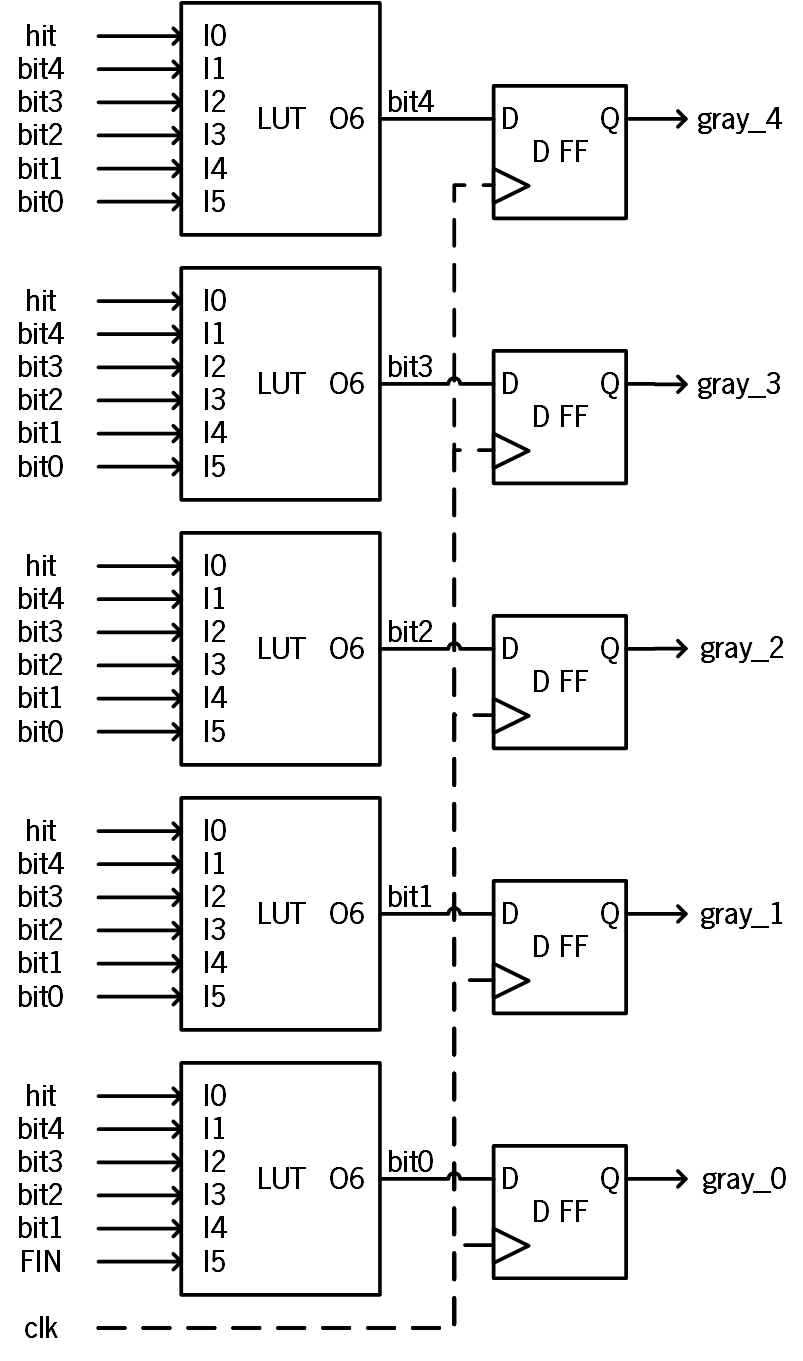
\includegraphics[width=.35\textwidth]{img/02_StateofArt/gray_code_first.png}
	\caption{Gray code oscillator TDC (adapted from \citep{gray_code_first} and \citep{gray_code_machado}).}
	\label{fig:gray_code_fisrt}
\end{figure}

\citet{gray_code_machado} proposed an improved version of the gray code oscillator \gls{TDC} that incorporates manual routing to improve linearity and precision. This reduces the need for calibration mechanisms and enables the use of the same calibration mechanism across multiple channels. The proposed architecture achieved a 380~ps resolution and a maximum \gls{DNL} of 0.38~\gls{LSB} and a \gls{INL} of 0.69~\gls{LSB}.It also uses only 16~\gls{FPGA} logic resources per channel. The main difference between this architecture and the previous one is the use of an external binary counter to extend the measurement range of the fine measurement stage, simplifying its design. Figure~\ref{fig:gray_code_rui} depicts the gray code oscillator schematic of a \gls{TDC} channel. The gray code counter is used to implement the \gls{TDC} channel for start and stop times, providing the system fine measurement. An input stage is also included to reduce power consumption by ensuring that the gray counters are only enabled for a single system clock cycle. The Merge Block concatenates the values from the coarse measurement and both \gls{TDC} channels.

\begin{figure}[ht!]
    \centering
  	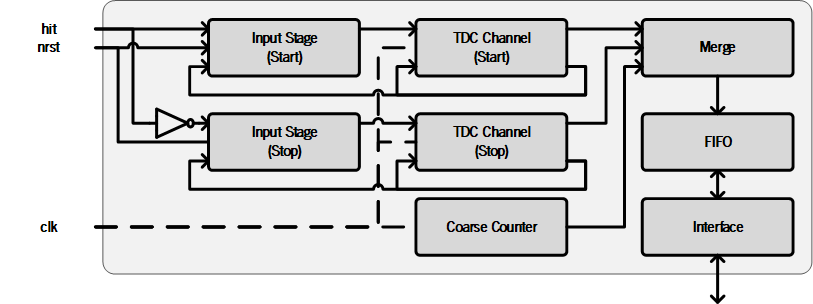
\includegraphics[width=0.7\textwidth]{img/02_StateofArt/gray_code_rui_bd.png}
    \caption{Gray code TDC block diagram (adapted from \citep{gray_code_machado}).}
    \label{fig:gray_code_rui}
\end{figure}

In \citeyear{gray_code_araujo}, \citet{gray_code_araujo} presents a gray code \gls{TDC} architecture that incorporates a double-sampling to improve resolution and precision. The second sampling stage is routed with a delay that is at least the double that of the first stage, allowing for the previous gray code value to be stored in the second stage when a new value arrives at the first stage. After the delay difference, the new value arrives at the second stage, resulting in both stages containing the same value. Adding the values from both stages produces an incremental sequence with improved resolution. Using a Zynq Ultrascale+ MPSoC, the proposed \gls{TDC} achieved a 69~ps resolution and a 59~ps precision using only 7 \glspl{LUT} and 20~\glspl{FF}, with a maximum \gls{DNL} and \gls{INL} of 1.76~\glspl{LSB} and 1.50~\glspl{LSB}, respectively. The architecture is scalable, allowing for multiple \gls{TDC} channels to be implemented by replicating a single channel's placement and routing. Figure~\ref{fig:gray_code_simao} shows the double-sampling gray \gls{TDC} channel schematic.

\begin{figure}[ht!]
	\centering
	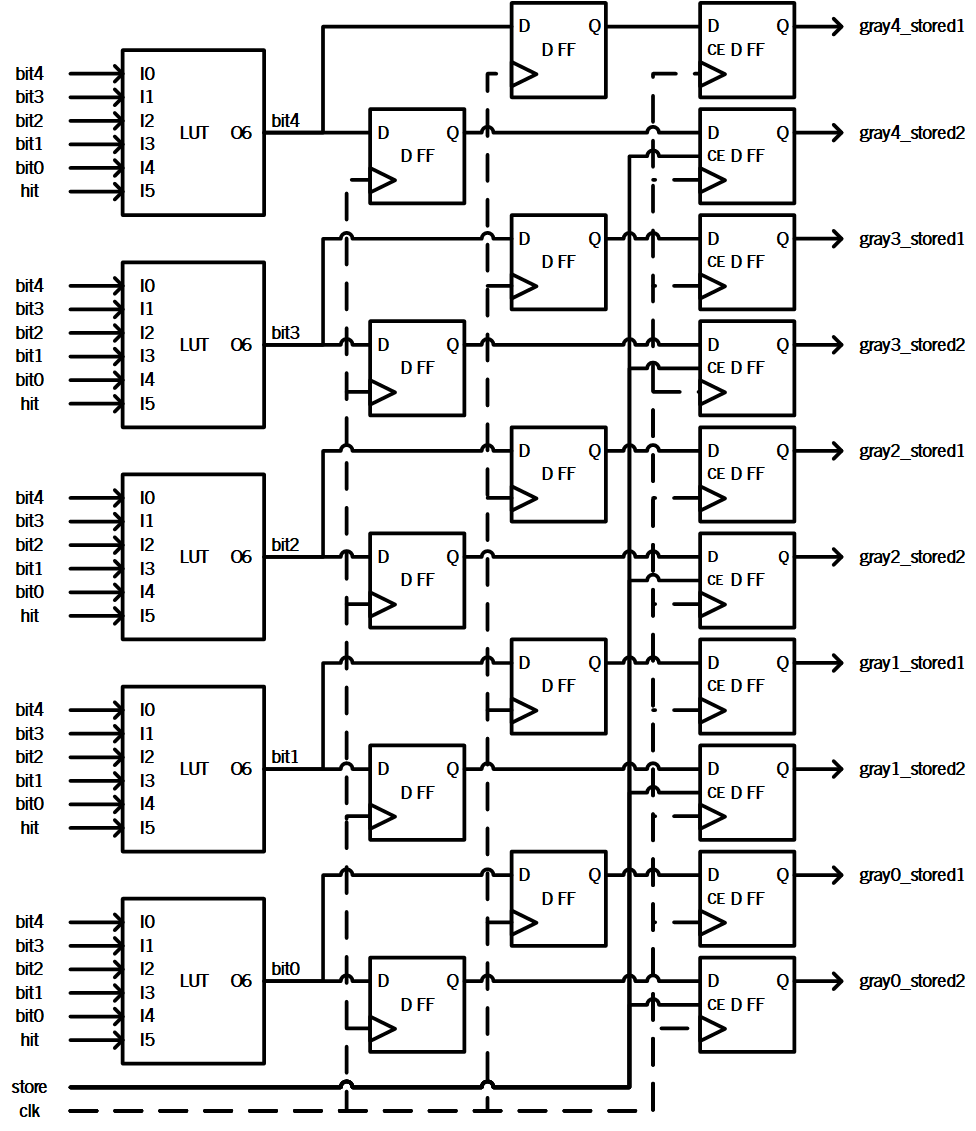
\includegraphics[width=.55\textwidth]{img/02_StateofArt/gray_code_simao.png}
	\caption{Double-sampling gray code TDC channel schematic (adapted from \citep{gray_code_araujo}).}
	\label{fig:gray_code_simao}
\end{figure}

\label{sub:gray_code}

% subsection gray_code (end)